%%%%%%%%%%%%%%%%%%%%%%%%%%%%%%%%%%%%%%%%%%%%%%%%%%%%%%%%%%%%%%%%%%%%%%%
% Author: Miguel Ferreira e Vanessa Silva                             %
% Info:                                                               %
% Language: Portuguese                                                %
%%%%%%%%%%%%%%%%%%%%%%%%%%%%%%%%%%%%%%%%%%%%%%%%%%%%%%%%%%%%%%%%%%%%%%%

\documentclass[a4paper,11pt,pdftex]{article}
\usepackage[T1]{fontenc}
\usepackage[portuguese]{babel}
\usepackage[utf8]{inputenc}
\usepackage{fullpage}
\usepackage[top=2.5cm, bottom=2.5cm, left=2.5cm , right=2.5cm]{geometry}
\usepackage{marginnote}        %use \marginnote{}
\usepackage[pdftex]{graphicx}  %Support for images in pdf
\usepackage{hyperref} 	       %Support for hyperlinks in pdf
\usepackage{textcomp}
\usepackage{tikz}
%\usepackage{times}            %times font
\usepackage{pdfpages} % Include a pdf page
\usepackage{caption}
\usepackage{subcaption}
\usepackage{verbatim}
\usepackage{color}
\usepackage{listings}          %for simple inclusion of source code
\usepackage[cc]{titlepic}      %glider on title page
\usepackage{url}
%\usepackage{natbib}
\usepackage{rotating}
\usepackage{lipsum}
\usepackage{fancyhdr}
\usepackage[português,ruled]{algorithm2e}
\usepackage[noend]{algpseudocode}
\usepackage{footnote}
\usepackage{amsfonts}
\usepackage{mathtools}
\definecolor{dkgreen}{rgb}{0,0.6,0}
\definecolor{gray}{rgb}{0.5,0.5,0.5}
\definecolor{mauve}{rgb}{0.58,0,0.82}
\definecolor{lightgrey}{RGB}{238,238,238}

\usepackage{enumerate}

%%%%%%%%%%%%%%%%%%%%IMPORTANTE COMMANDS I FORGET%%%%%%%%%%%%%%%%%%%%%%%
% \marginnote                                                         %
% \footnote                                                           %
% \hiperlink{tag}{text} & hypertarget{tag}{text}                      %
%%%%%%%%%%%%%%%%%%%%%%%%%%%%%%%%%%%%%%%%%%%%%%%%%%%%%%%%%%%%%%%%%%%%%%%
% [hidelinks] doesn't work so:                                        %
%                                                                     %
%  \hypersetup{                                                       %
%   colorlinks=false,                                                 %
%  pdfborder={0 0 0},                                                 %
%  }                                                                  %
% \framebox[\linewidth][l]{                                           %
% \lstinputlisting[title=HelloWorld.c]{./Programs/HelloWorld.c}       %
% }                                                                   %
%\includepdf[pages={{},{1},{},{2},{},{3},{},{4},{},{5},{},{6},{},{7}, %
%{},{8},{},{9},{},{10},{},{11},{},{12}},pagecommand={\thispagestyle{  %
% fancy}}]{script}                                                    %
%%%%%%%%%%%%%%%%%%%%%%%%%%%%%%%%%%%%%%%%%%%%%%%%%%%%%%%%%%%%%%%%%%%%%%%

\title{Trabalho 1 - Encaminhamento Estático}

\author{Miguel Ferreira\\
  \href{mailto:miguelferreira108@gmail.com}{\texttt{miguelferreira108@gmail.com}}\\
  Vanessa Silva\\
  \href{mailto:up201305731@fc.up.pt}{\texttt{up201305731@fc.up.pt}}\\
\multicolumn{1}{p{.7\textwidth}}{\centering\emph{
Administração de Redes,\\Departamento de Ciências de Computadores,\\Faculdade de Ciências da Universidade do Porto}}
}
\date{\today}
%\titlepic{
%}

%%%%%%%%%%%%%%%%%%%%%%%%%%%%% SETTINGS %%%%%%%%%%%%%%%%%%%%%%%%%%%%%%%%
\lstset{
  language=C,   % choose the language of the code
  numbers=left,        % where to put the line-numbers
  stepnumber=1,        % the step between two line-numbers.        
  numbersep=8pt,       % how far the line-numbers are from the code
  backgroundcolor=\color{lightgrey}, % \usepackage{color}
  showspaces=false,    % show spaces adding particular underscores
  showstringspaces=false,        % underline spaces within strings
  showtabs=false,      % show tabs within strings adding underscores
  tabsize=2,           % sets default tabsize to 2 spaces
  captionpos=b,        % sets the caption-position to bottom
  breaklines=true,     % sets automatic line breaking
  breakatwhitespace=true, % if automatic breaks only happen atwhitespace
  title=\lstname,      % show the filename of files \lstinputlisting;
  frame=single,
  keywordstyle=\color{blue},          % keyword style
  commentstyle=\color{dkgreen},       % comment style
  stringstyle=\color{mauve},
  basicstyle=\ttfamily,
}
\hypersetup{
    bookmarks=true,         % show bookmarks bar?
    unicode=true,          % non-Latin characters in Acrobat’sbookmarks
    pdftoolbar=true,        % show Acrobat’s toolbar?
    pdfmenubar=true,        % show Acrobat’s menu?
    pdffitwindow=false,     % window fit to page when opened
    pdfstartview={FitH},    % fits the width of the page to the window
    pdftitle={Título},    % title
    pdfauthor={Miguel Ferreira e Vanessa Silva},                        % author
    pdfcreator={Miguel Ferreira e Vanessa Silva},   % creator of the document
%     pdfproducer={Producer}, % producer of the document
%     pdfkeywords={keyword1} {key2} {key3}, % list of keywords
%     pdfnewwindow=true,      % links in new window
%     colorlinks=false,       % false: boxed links; true: colored links
%     linkcolor=red,          % color of internal links
%     citecolor=green,        % color of links to bibliography
%     filecolor=magenta,      % color of file links
%     urlcolor=cyan           % color of external links
}

%%%%%%%%%%%%%%%%%%%%%%%%%% END SETTINGS %%%%%%%%%%%%%%%%%%%%%%%%%%%%%%%
\begin{document}
\maketitle
%\tableofcontents
\section*{Introdução}

No âmbito da unidade curricular de Administração de Redes, implementamos a rede descrita na figura \ref{fig:rede}.

\begin{figure}[h]
\centering
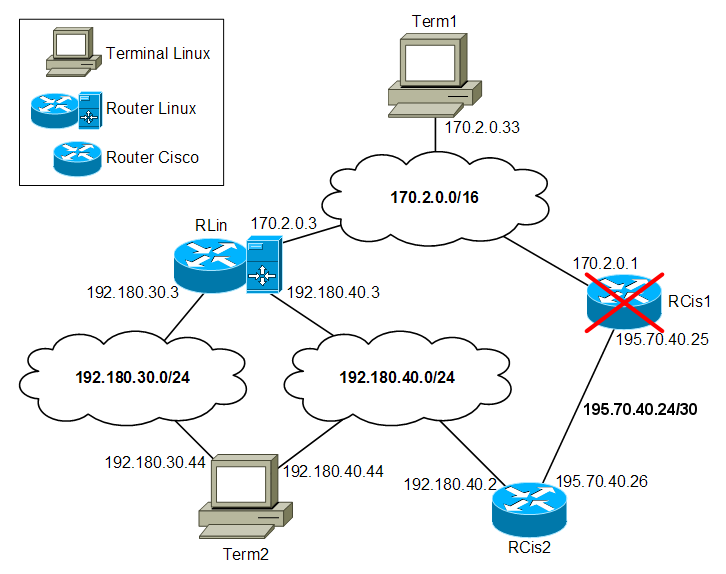
\includegraphics[width=0.7\textwidth]{rede.png}
\label{fig:rede}
\caption{Rede implementada na aula.}
\end{figure}

As máquinas \textsf{Term1}, \textsf{Term2} e \textsf{RLin} foram concretizadas com 3 \emph{workstations} Fedora 23, cada uma com as necessárias interfaces de rede. A máquina \textsf{RCis2} consiste num \emph{router} Cisco 1841.

A rede \textsf{170.2.0.0/16} consiste na ligação direta entre uma interface de \textsf{RLin} e \textsf{Term1}.
A rede \textsf{192.180.30.0/24} foi implementada com uma ligação direta entre \textsf{RLin} e \textsf{Term2}.
A rede \textsf{192.180.40.0/24} foi implementada com um \emph{switch} ligado a \textsf{RLin}, \textsf{Term2} e \textsf{RCis2}. 

\section{Conectividade}
\paragraph{a)}
\begin{verbatim}
root@localhost ar]# traceroute -n -N 1 192.180.30.3
traceroute to 192.180.30.3 (192.180.30.3), 30 hops max, 60 byte packets
 1  192.180.30.3  0.458 ms  0.189 ms  0.187 ms
[root@localhost ar]# traceroute -n -N 1 192.180.40.3
traceroute to 192.180.40.3 (192.180.40.3), 30 hops max, 60 byte packets
 1  192.180.40.3  0.557 ms  0.071 ms  0.064 ms
[root@localhost ar]# traceroute -n -N 1 170.2.0.3
traceroute to 170.2.0.3 (170.2.0.3), 30 hops max, 60 byte packets
 1  192.180.40.2  0.462 ms 0.366 ms 0.382 ms
 2  * * *
 3  * * *
 4  * * *
 5  *
\end{verbatim}

\paragraph{b)}
\begin{verbatim}
[root@localhost ar]# traceroute -n -N 1 192.180.40.44                    
traceroute to 192.180.40.44 (192.180.40.44), 30 hops max, 60 byte packets
 1  170.2.0.33  3005.124 ms !H  3005.860 ms !H  3005.921 ms !H           
[root@localhost ar]# traceroute -n -N 1 192.180.30.44                    
traceroute to 192.180.30.44 (192.180.30.44), 30 hops max, 60 byte packets
 1  170.2.0.3  0.331 ms  0.225 ms  0.233 ms                              
 2  * * *                                                                
 3  * * *                                                                
 4  * * *                                                                
 5  *                                                                    
\end{verbatim}

\subparagraph{i)}
\begin{verbatim}
[root@localhost ar]# traceroute -n -N 1 192.180.40.44                     
traceroute to 192.180.40.44 (192.180.40.44), 30 hops max, 60 byte packets 
 1  170.2.0.33  3005.124 ms !H  3005.860 ms !H  3005.921 ms !H            
[root@localhost ar]# traceroute -n -N 1 192.180.30.44                     
traceroute to 192.180.30.44 (192.180.30.44), 30 hops max, 60 byte packets 
 1  170.2.0.3  0.331 ms  0.225 ms  0.233 ms                               
 2  * * *                                                                 
 3  * * *                                                                 
 4  * * *                                                                 
 5  * * *                                                                 
 6  * * *                                                                 
\end{verbatim}
\subparagraph{ii)}
Comandos Cisco:
\begin{verbatim}                                                         
router_g04>enable                                                        
router_g04#config                                                        
Configuring from terminal, memory, or network [terminal]?                
Enter configuration commands, one per line.  End with CNTL/Z.            
router_g04(config)#ip route 170.2.0.0 255.255.0.0 195.70.40.25           
router_g04(config)#end                                                   
\end{verbatim}                                                                                                                                               
Terminal:
\begin{verbatim}                                                                         
[root@localhost ar]# traceroute -n -N 1 192.180.40.44                    
traceroute to 192.180.40.44 (192.180.40.44), 30 hops max, 60 byte packets
 1  170.2.0.33  3004.524 ms !H  3005.865 ms !H  3005.837 ms !H           
[root@localhost ar]# traceroute -n -N 1 192.180.30.44                    
traceroute to 192.180.30.44 (192.180.30.44), 30 hops max, 60 byte packets
 1  170.2.0.3  0.330 ms  0.071 ms  0.068 ms                                                             
 2  * * *                                                                
 3  * * *                                                                
 4  * * *                                                                
 5  * * *                                                                
 6  * * *                                                                
 7  * * *                                                                
\end{verbatim}
\subparagraph{iii)}
Comandos Cisco:
\begin{verbatim}                                                         
router_g04>enable                                                        
router_g04#config                                                        
Configuring from terminal, memory, or network [terminal]?                
Enter configuration commands, one per line.  End with CNTL/Z.            
router_g04(config)#ip route 170.2.0.0 255.255.0.0 192.180.40.3           
router_g04(config)#end                                                   
\end{verbatim}                                                          
Terminal:
\begin{verbatim}
[root@localhost ar]# traceroute -n -N 1 192.180.40.44                    
traceroute to 192.180.40.44 (192.180.40.44), 30 hops max, 60 byte packets
 1  170.2.0.33  3005.787 ms !H  3005.895 ms !H  3005.845 ms !H           
[root@localhost ar]# traceroute -n -N 1 192.180.30.44                    
traceroute to 192.180.30.44 (192.180.30.44), 30 hops max, 60 byte packets
 1  170.2.0.3  0.115 ms  0.067 ms  0.067 ms                              
 2  192.180.30.44  0.406 ms  0.684 ms  0.303 ms                                                                             
\end{verbatim}

\paragraph{c)}
Na alínea \it{b} pretendemos testar a conectividade entre as máquinas \textsf{Term1} e \textsf{Term2}.
Em \it{b i} os pacotes chegam à máquina \textsf{Term2} pela interface enp1s6 (192.180.30.44) que envia os pacotes, como resposta, pela interface enp0s7 (192.180.40.44) para o \emph{router} \textsf{RCis2} (192.180.40.2), uma vez que é a sua rota por defeito, como \textsf{RCis2} não tem rota para a rede 170.2.0.0/16 os pacotes são perdidos.
Em \it{b ii} os pacotes chegam a \textsf{Term2} pela interface enp1s6 (192.180.30.44) que envia os pacotes, como resposta, pela interface enp0s7 (192.180.40.44) para o \emph{router} \textsf{RCis2}, (rota por defeito), como este é configurado com uma rota para a rede 170.2.0.0/16 através de \textsf{RCis1}, que é um \emph{router} fisicamente inexistente, a resposta nunca chega a \textsf{Term1}.
Em \it{b iii} o percurso dos pacotes é idêntico ao descrito para a alínea \it{b ii}, à exceção de que, neste caso, o \emph{router} \textsf{RCis2} é configurado com uma rota para a rede 170.2.0.0/16 através da máquina \textsf{RLin}. \textsf{RCis2} envia então os pacotes para \textsf{RLin} (192.180.40.3) que reenvia-os para a máquina de origem.
Em todos os casos, \it{b i}, \it{b ii} e \it{b iii}, quando a máquina \textsf{Term1} envia os pacotes para a interface enp0s7, que tem o endereço IP 192.180.40.44, os pacotes não chegam ao destino. Isto acontece pois \textsf{Term1} tem uma rota para a rede 192.180.40.0/24 através de \textsf{RCis1}, que é um \emph{router} fisicamente inexistente.
\newpage
Rotas da máquina \textsf{Term1}:
\begin{verbatim}
[root@localhost ar]# route -n
Kernel IP routing table
Destination     Gateway         Genmask         Flags Metric Ref    Use Iface
0.0.0.0         170.2.0.3       0.0.0.0         UG    0      0        0 enp0s7
169.254.0.0     0.0.0.0         255.255.0.0     U     1002   0        0 enp0s7
170.2.0.0       0.0.0.0         255.255.0.0     U     0      0        0 enp0s7
192.180.40.0    170.2.0.1       255.255.255.0   UG    0      0        0 enp0s7
\end{verbatim}

Rotas da máquina \textsf{Term2}:
\begin{verbatim}
[root@localhost ar]# route -n
Kernel IP routing table
Destination     Gateway         Genmask         Flags Metric Ref    Use Iface
0.0.0.0         192.180.40.2    0.0.0.0         UG    0      0        0 enp0s7
169.254.0.0     0.0.0.0         255.255.0.0     U     1002   0        0 enp0s7
169.254.0.0     0.0.0.0         255.255.0.0     U     1003   0        0 enp1s6
192.180.30.0    0.0.0.0         255.255.255.0   U     0      0        0 enp1s6
192.180.40.0    0.0.0.0         255.255.255.0   U     0      0        0 enp0s7
\end{verbatim}

\paragraph{d)}
Como vimos, perante algumas condições estipuladas, os pacotes enviados da máquina \textsf{Term1} à \textsf{Term2} foram perdidos, ou não chegaram ao destino ou a resposta não chegou à origem.
No encaminhamento dinâmico, tal como o nome indica, as rotas (caminhos) são calculados dinamicamente recorrendo a protocolos de encaminhamento dinâmico que se adaptam a possíveis alterações que acontecem na rede. Estes protocolos envolvem a troca de informação de controlo entre os nós (terminais e \emph{routers}) encaminhadores, são desenvolvidos para trocar para uma rota alternativa quando a rota primária se torna inoperável e para decidir qual é a melhor rota para o destino.
Com este tipo de encaminhamento os pacotes perdidos, muito provavelmente, não seria perdidos, uma vez que os protocolos de encaminhamento dinâmico atualizam automaticamente as tabelas de encaminhamento dos \emph{routers}, de modo a encontrarem a rota ideal para chegar ao destino.

\paragraph{e)}
\subparagraph{i)}
\begin{verbatim}
[root@localhost ~]# traceroute -n -N 1 170.2.0.33
traceroute to 170.2.0.33 (170.2.0.33), 30 hops max, 60 byte packets
 1  192.180.40.3  0.093 ms  0.064 ms  0.063 ms                                                             
 2  * * *                                                                
 3  * * *                                                                
 4  * * *                                                                
 5  * * *                                                                
 6  * *
\end{verbatim}
\subparagraph{ii)}
Comandos Cisco:
\begin{verbatim}
router_g04>enable
router_g04#config
Configuring from terminal, memory, or network [terminal]? 
Enter configuration commands, one per line.  End with CNTL/Z.
router_g04(config)#ip route 170.2.0.0 255.255.0.0 195.70.40.25
router_g04(config)#end
\end{verbatim}
Terminal:
\begin{verbatim}
[root@localhost ~]# traceroute -n -N 1 170.2.0.33
traceroute to 170.2.0.33 (170.2.0.33), 30 hops max, 60 byte packets
 1  192.180.40.3  0.294 ms  0.165 ms  0.072 ms                                                             
 2  * * *                                                                
 3  * * *                                                                
 4  * * *                                                                
 5  * * *                                                                
 6  * *
\end{verbatim}
\subparagraph{iii)}
Comandos Cisco:
\begin{verbatim}
router_g04>enable
router_g04#config
Configuring from terminal, memory, or network [terminal]? 
Enter configuration commands, one per line.  End with CNTL/Z.
router_g04(config)#ip route 170.2.0.0. 255.255.0.0
router_g04(config)#ip route 170.2.0.0 255.255.0.0 192.180.40.3 
router_g04(config)#end
\end{verbatim}
Terminal:
\begin{verbatim}
[root@localhost ~]# traceroute -n -N 1 170.2.0.33
traceroute to 170.2.0.33 (170.2.0.33), 30 hops max, 60 byte packets
 1  192.180.40.3  0.307 ms  0.247 ms  0.065 ms  
 2  * * *                                                                
 3  * * *                                                                
 4  * * *                                                                
 5  * * *                                                                
 6  * *
\end{verbatim}

\paragraph{f)}
Sim, seria útil ter encaminhamento dinâmico nos \emph{routes}, pois mais uma vez vemos que os pacotes, em \it{e i} e \it{e ii}, perdem-se, e em \it{e iii} chegam ao destino mas, neste caso a resposta é enviada para o \emph{router} \textsf{RCis1} que não existe fisicamente e por isso também se perdem. Com o encaminhamento dinâmico os \emph{routers} escolhiam sempre a melhor rota, como explicado na alínea \it{d}, de modo a que estes problemas se resolvessem.

\paragraph{g)}
\subparagraph{i)}
\begin{verbatim}
[root@localhost ar]# traceroute -n -N 1 170.2.0.15
traceroute to 170.2.0.15 (170.2.0.15), 30 hops max, 60 byte packets
 1  192.180.40.2  0.491 ms  0.376 ms  0.384 ms
 2  192.180.40.3  0.601 ms  3005.145 ms !H  3005.706 ms !H
[root@localhost ar]# traceroute -n -N 1 170.2.0.15
traceroute to 170.2.0.15 (170.2.0.15), 30 hops max, 60 byte packets
 1  192.180.40.3  0.100 ms  0.070 ms  0.069 ms
 2  192.180.40.3  3005.710 ms !H  3005.788 ms !H  3005.939 ms !H
\end{verbatim}

\begin{figure}[h]
\centering
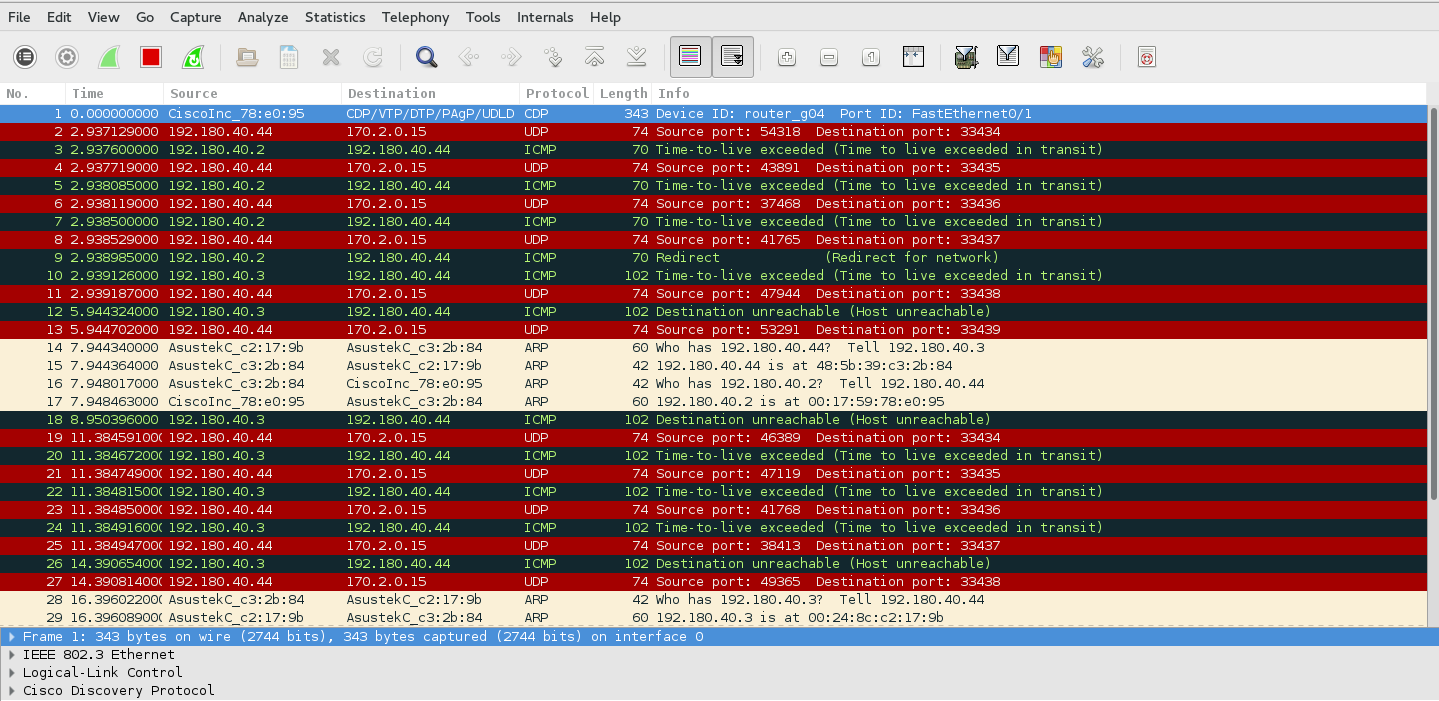
\includegraphics[width=0.9\textwidth, height=0.35\textheight]{1_g1_screenshot.png}
\label{fig:wireshark-enp0s7}
\caption{\emph{Screenshot} da captura de pacotes na interface enp0s7 (IP 192.180.40.44) no \emph{wireshark}.}
\end{figure}
\newpage
\subparagraph{ii)}
(a fazer).
\section{ARP}
\paragraph{a}

\begin{figure}[h]
\centering
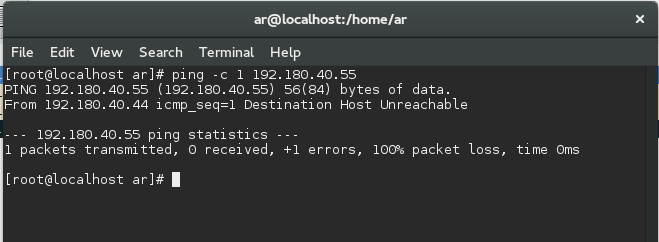
\includegraphics[width=0.7\textwidth]{2_a_screenshot.png}
\label{fig:ping}
\caption{Resultado de \textsf{ping -c 1 192.180.40.55}.}
\end{figure}

\paragraph{b}
Como podemos verificar no \emph{screenshot} abaixo, capturou-se 3 pacotes ARP de modo a "resolver" o endereço IP 192.180.40.55. Entre as tentativas houve um \emph{timeout} de aproximadamente 1 segundo, uma vez que entre elas (retransmissões) não se conseguiu "resolver" o endereço IP e, depois da terceira tentativa sem resposta, é enviado um pacote ICMP \emph{Host Unreachable} ao IP de origem.
É, exatamente, desta forma que funciona o protocolo ARP, ou seja, quando a tradução de um endereço IP não se encontra na cache de ARP é necessário "resolver" esse endereço. Para tal, é enviado uma trama para o endereço MAC de difusão (pacote ARP), todos os nós (terminais e/ou \emph{routers}) recebem e processam a trama, mas apenas o que reconhece o endereço pretendido responde e a informação é adicionada à cache de ARP. Se não ocorrer a resposta no espaço de 1 segundo (\emph{timeout}), a trama é retransmitida e, se à \textbf{terceira} tentativa não receber resposta, "desiste" e é enviado um ICMP \emph{Host Unreachable} (!H) ao IP de origem do pacote.

\begin{figure}[h]
\centering
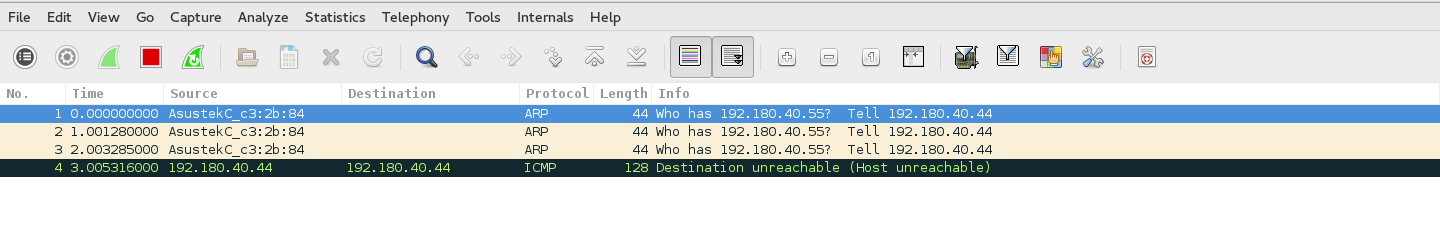
\includegraphics[width=0.7\textwidth]{2_a__screenshot.png}
\label{fig:wireshark}
\caption{\emph{Screenshot} do \emph{wireshark} a correr na máquina \textsf{Term2}.}
\end{figure}
\section{Captura}
\paragraph{a)}
Comando com o filtro de captura pretendido:
\begin{verbatim}
tcpdump -nn 'tcp[tcpflags] & tcp-push == tcp-push' and 'ip[2:2] < 128' > ssh.dump
\end{verbatim}

O resultado da captura é o seguinte:
\begin{verbatim}
  11:00:59.019099 IP 170.2.0.33.41460 > 192.180.30.44.22: Flags [P.],
seq 3235348810:3235348854, ack 1796210900, win 288, options [nop,nop,
TS val 2288580 ecr 2411765], length 44
  11:00:59.503156 IP 170.2.0.33.41460 > 192.180.30.44.22: Flags [P.], 
seq 44:80, ack 93, win 288, options [nop,nop,TS val 2289064 ecr 2470611], length 36
  11:00:59.503611 IP 192.180.30.44.22 > 170.2.0.33.41460: Flags [P.], seq 93:129, 
ack 80, win 340, options [nop,nop,TS val 2471095 ecr 2289064], length 36
  11:00:59.503638 IP 192.180.30.44.22 > 170.2.0.33.41460: Flags [P.], seq 129:173, 
ack 80, win 340, options [nop,nop,TS val 2471095 ecr 2289064], length 44
  11:01:00.504865 IP 192.180.30.44.22 > 170.2.0.33.41460: Flags [P.], seq 173:217, 
ack 80, win 340, options [nop,nop,TS val 2472096 ecr 2289064], length 44
  11:01:01.505841 IP 192.180.30.44.22 > 170.2.0.33.41460: Flags [P.], seq 217:261, 
ack 80, win 340, options [nop,nop,TS val 2473097 ecr 2290066], length 44
  11:01:02.506759 IP 192.180.30.44.22 > 170.2.0.33.41460: Flags [P.], seq 261:305, 
ack 80, win 340, options [nop,nop,TS val 2474098 ecr 2291067], length 44
  11:01:03.507958 IP 192.180.30.44.22 > 170.2.0.33.41460: Flags [P.], seq 305:349, 
ack 80, win 340, options [nop,nop,TS val 2475099 ecr 2292068], length 44
  11:01:04.508887 IP 192.180.30.44.22 > 170.2.0.33.41460: Flags [P.], seq 349:393, 
ack 80, win 340, options [nop,nop,TS val 2476100 ecr 2293069], length 44
  11:01:05.509815 IP 192.180.30.44.22 > 170.2.0.33.41460: Flags [P.], seq 393:437, 
ack 80, win 340, options [nop,nop,TS val 2477101 ecr 2294070], length 44
  11:01:06.510972 IP 192.180.30.44.22 > 170.2.0.33.41460: Flags [P.], seq 437:481, 
ack 80, win 340, options [nop,nop,TS val 2478102 ecr 2295071], length 44
  11:01:07.511956 IP 192.180.30.44.22 > 170.2.0.33.41460: Flags [P.], seq 481:533, 
ack 80, win 340, options [nop,nop,TS val 2479103 ecr 2296072], length 52
  11:01:07.881220 IP 170.2.0.33.41460 > 192.180.30.44.22: Flags [P.], seq 80:116, 
ack 533, win 288, options [nop,nop,TS val 2297442 ecr 2479103], length 36
  11:01:07.881675 IP 192.180.30.44.22 > 170.2.0.33.41460: Flags [P.], seq 533:569, 
ack 116, win 340, options [nop,nop,TS val 2479473 ecr 2297442], length 36
  11:01:07.881775 IP 192.180.30.44.22 > 170.2.0.33.41460: Flags [P.], seq 569:605, 
ack 116, win 340, options [nop,nop,TS val 2479473 ecr 2297442], length 36
  11:01:07.881861 IP 192.180.30.44.22 > 170.2.0.33.41460: Flags [P.], seq 605:665, 
ack 116, win 340, options [nop,nop,TS val 2479473 ecr 2297442], length 60
  11:01:07.882171 IP 192.180.30.44.22 > 170.2.0.33.41460: Flags [P.], seq 665:717, 
ack 116, win 340, options [nop,nop,TS val 2479473 ecr 2297443], length 52
\end{verbatim}
\newpage
\begin{figure}[h]
\centering
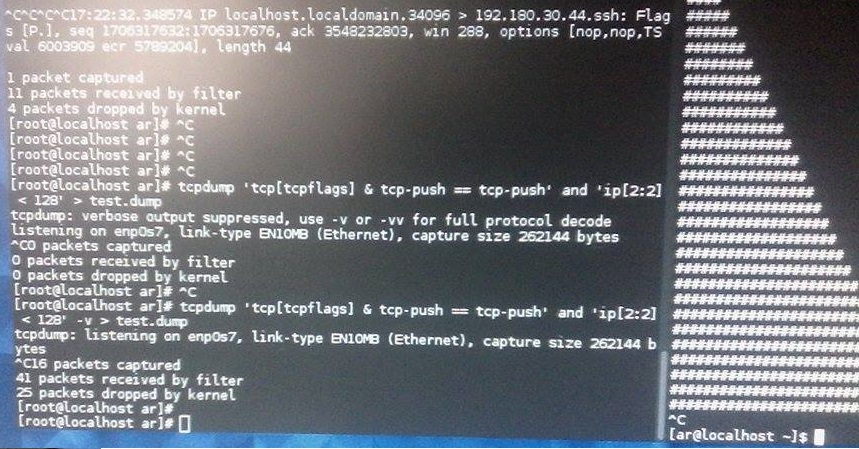
\includegraphics[width=0.8\textwidth]{3_a_filtro.png}
\label{fig:filtro}
\caption{Teste do filtro utilizado.}
\end{figure}

\begin{figure}[h]
\centering
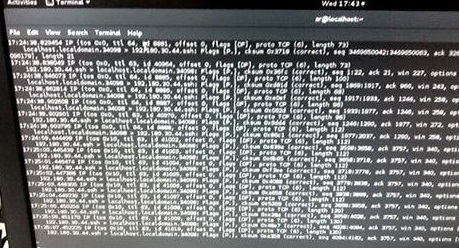
\includegraphics[width=0.8\textwidth]{3_a_resultado_do_tcpdump.png}
\label{fig:tcpdump}
\caption{Resultado do filtro de captura.}
\end{figure}

\paragraph{b)}
Filtro de visualização pretendido:
\begin{verbatim}
tcp.flags.push == 1 && ip.len < 128
\end{verbatim}
Na figura abaixo, podemos ver o resultado da captura, no \emph{wireshark}, usando este filtro.

\begin{figure}[h]
\centering
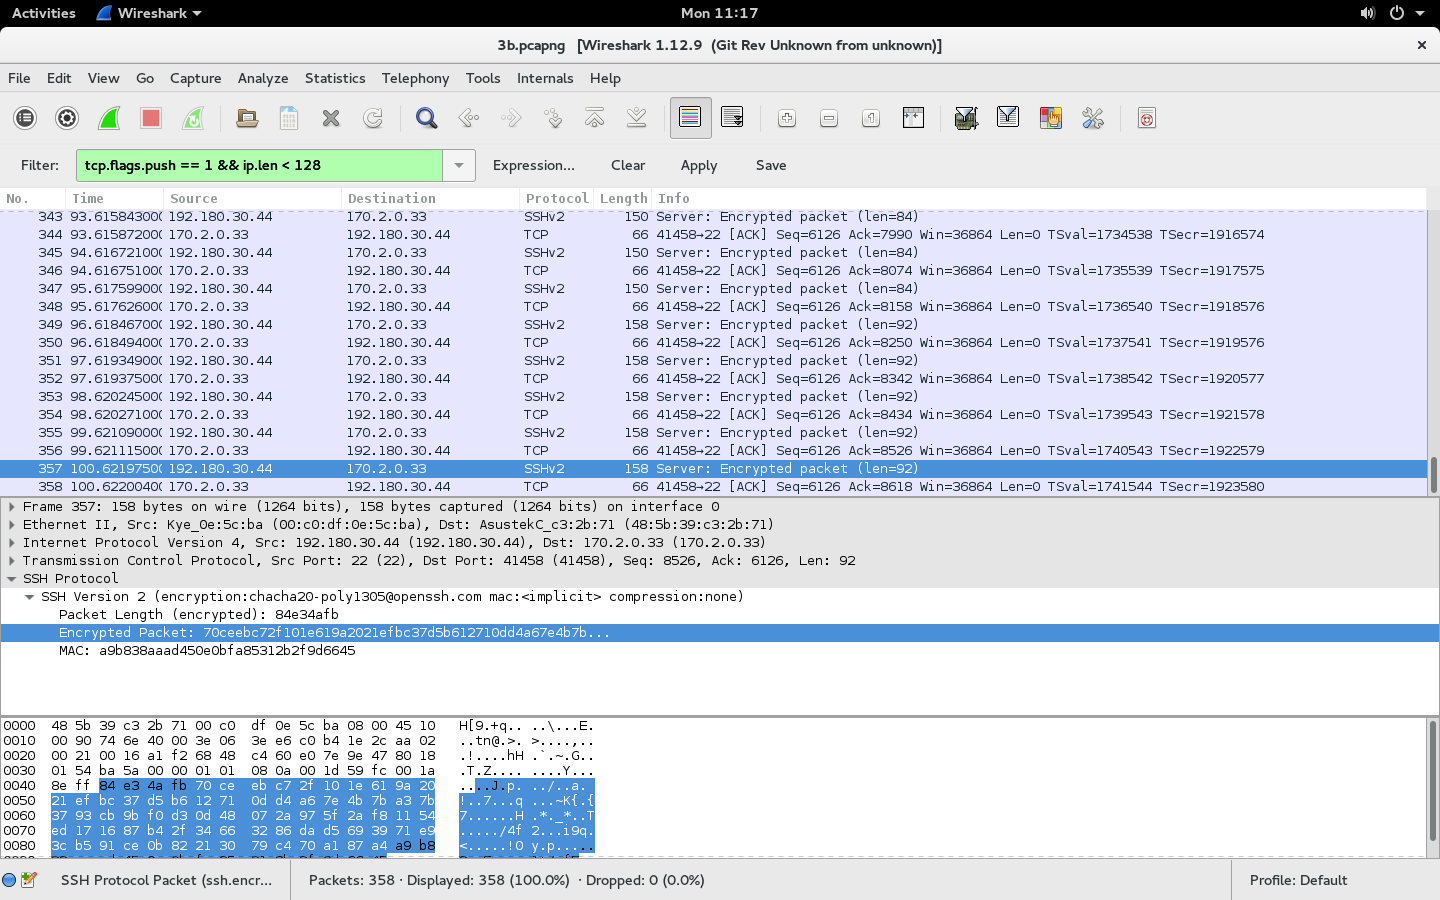
\includegraphics[width=0.95\textwidth, height=0.5\textheight]{3_b_screenshot.png}
\label{fig:wireshark}
\caption{Resultado do filtro de visualização do \emph{wireshark}.}
\end{figure}
\newpage
\paragraph{c)}
Para calcular o comprimento de um pacote IP subtrai-se o seu tamanho total (cabeçalho + dados), encontrado nos bytes 2 a 3 (indexado a 0), pelo comprimento do próprio cabeçalho, encontrado no primeiro byte, nos últimos 4 bits (mais à direita).
%\listoffigures
%\listoftables
%\listofalgorithms
\bibliographystyle{acm}
\bibliography{bibl}
\end{document}
